\section{Risultati}\label{sec:risultati}
I valori numerici dei coefficienti per i controller \textsc{lqr} e \textsc{pid} sono riportati in appendice \ref{sec:parametri-sistema}
rispettivamente in tabella \ref{tab:coefficienti-lqr} e \ref{tab:coefficienti-pid}.
Usando questi parametri, il pendolo rimane rovesciato (figura )%todo add foto
Tutto il codice usato per stabilizzare il pendolo e calcolare i parametri è disponibile sul mio GitHub\cite{github}.

Per avere un'idea concreta dei risultati, ho integrato il sistema usando entrambi i controller\footnote{Raccogliere
i dati del sistema fisico vero è possibile ma poco pratico. Integrando a computer ho dei grafici più chiari e, soprattutto,
confrontabili tra di loro (i.e. hanno le stesse condizioni iniziali).} (figure \ref{fig:int-lqr} e \ref{fig:int-pid}).
Il risultato è compatibile con quello che si osserva per il sistema reale.
Ho integrato anche $f^*f$ per entrambi i sistemi; il risultato è:
\begin{equation}
  \frac {E_{LQR} } {E_{PID}} \approx \frac 3 5
  \label{eq:rapporto-f}
\end{equation}

Aggiungo anche che, qualitativamente, ho osservato che il controller \textsc{lqr} funziona meglio del \textsc{pid}, ma
richiede che i dati in input dei sensori siano più \emph{puliti}.

\begin{figure}[h]
  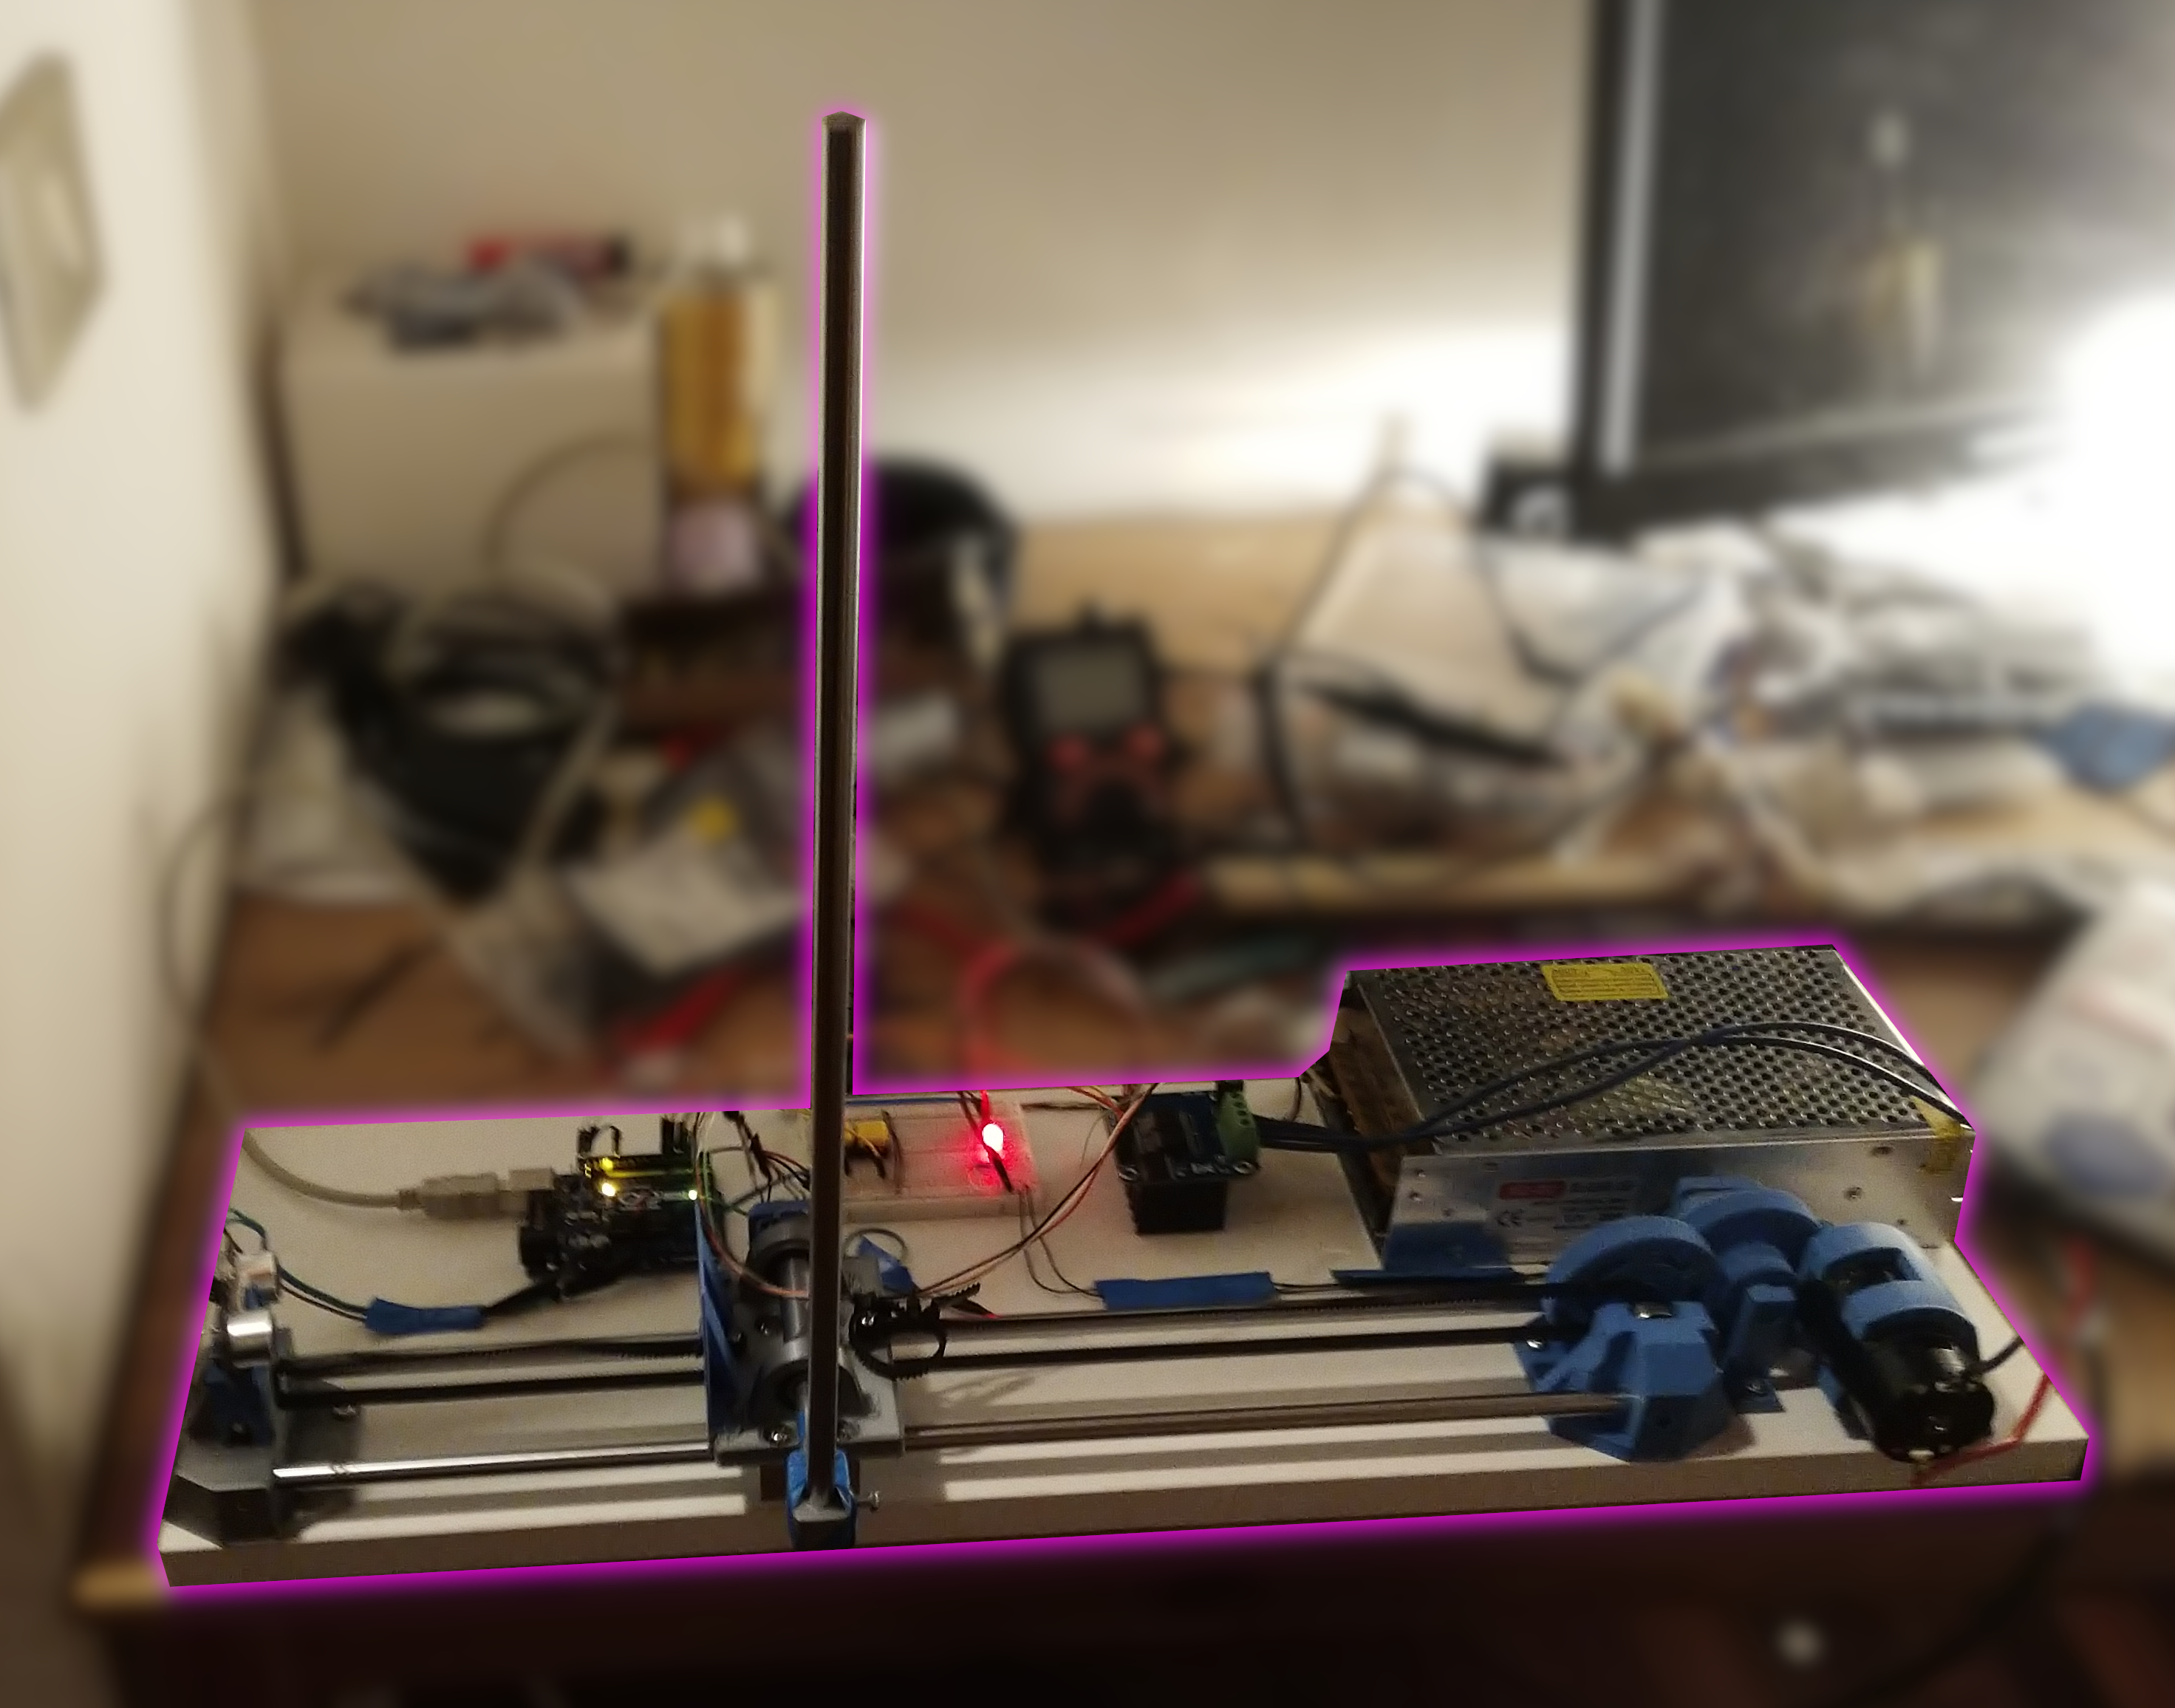
\includegraphics[width=0.5\textwidth]{pend-up.jpg}
  \caption{\emph{Sistema del pendolo invertito stabilizzato.}}
  \label{fig:pend-up}
\end{figure}

\begin{figure}[h]
  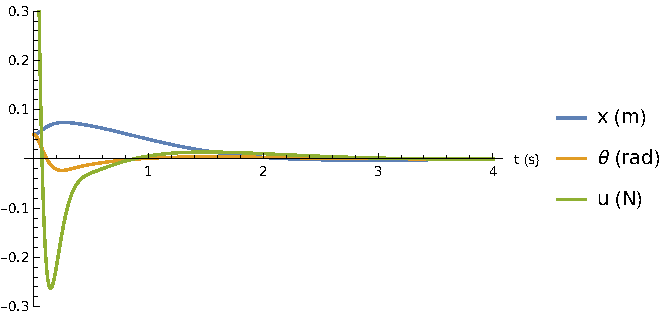
\includegraphics[width=0.47\textwidth]{integrazione lqr.pdf}
  \caption{\emph{Sistema controllato con LQR; il controller lineare è applicato alle equazioni vere del moto.}}
  \label{fig:int-lqr}
\end{figure}

\begin{figure}[h]
  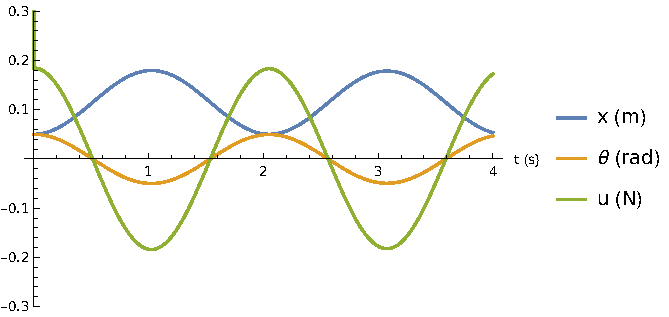
\includegraphics[width=0.47\textwidth]{integrazione pid.pdf}
  \caption{\emph{Sistema controllato con PID; il controller è applicato alle equazioni vere del moto.}}
  \label{fig:int-pid}
\end{figure}



